\documentclass{beamer}
\usetheme{metropolis}
\usepackage{graphicx}
\usepackage{amsmath}
\usepackage{tcolorbox}
\title{Electromagnetic Theory: Special Presentation}
\author{Jordan Hanson}
\institute{Whittier College Department of Physics and Astronomy}

\def\rcurs{{\mbox{$\resizebox{.16in}{.08in}{
\includegraphics{ScriptR}}$}}}
\def\brcurs{{\mbox{$\resizebox{.16in}{.08in}{
\includegraphics{BoldR}}$}}}
\def\hrcurs{{\mbox{$\hat \brcurs$}}}
\DeclareMathOperator{\sign}{sign}

\begin{document}
\maketitle

\section{Outline}

\begin{frame}{Outline}
\begin{enumerate}
\item The continuous limit
\begin{itemize}
\item How accurate is the idea that $\Delta x \sum_i q_i \rightarrow \int dq$?
\item The spatial Fourier transform
\end{itemize}
\item The line of charges
\begin{itemize}
\item Discrete, continuous
\item Far-field approximation to third order in $(1/r)^n$
\item Spatial Fourier transforms
\end{itemize}
\end{enumerate}
\end{frame}

\section{The Continuous Limit}

\begin{frame}{The Continuous Limit}
\alert{\textbf{The continuous limit:}} Why do we speak of macroscopic fields from fluid charge distributions?  We know that charge is \textit{discrete.}
\rule{10cm}{0.25pt}
\alert{\textbf{The continuous limit:}} Why do we speak of macroscopic fluids from fluid mass distributions?  We know that mass is \textit{discrete.}
\small
\begin{enumerate}
\item Consider a row of $2N + 1$ point charges $q$ along the $x$-axis, separated by $\Delta x$.  Why $2N + 1$?  Place $N$ on either side of the origin, and one at the origin.  Let $P$ be a distance $z$ above the origin along the z-axis.
\item Consider concentric rings of point charges $q$ along the $\phi$-axis in cylindrical coordinates.  Each ring is at some radius $s$ from the origin.  The separations are therefore $\Delta \phi$ and $\Delta s$, and there is one charge at the origin.
\end{enumerate}
\end{frame}

\begin{frame}{The Continuous Limit}
\alert{\textbf{Project goals:}}
\begin{enumerate}
\item Obtain discrete and continuous results to $\mathcal{O}(1/r)^3$
\item Calculate spatial Fourier transform of each result
\end{enumerate}
The spatial Fourier transform relates position $x$ with wavenumber $k = 2\pi/\lambda$ (inverse length units). The spatial Fourier transform of a function $f(z)$ is defined:
\begin{align}
\widetilde{f}(k) &= \int_{-\infty}^{\infty} f(x) e^{-2\pi i k z} dz \\
f(x) &= \int_{-\infty}^{\infty} \widetilde{f}(k) e^{2\pi i k z} dk
\end{align}
\end{frame}

\section{The Line of Charges}

\begin{frame}{The Line of Charges}
\small
\begin{figure}
\centering
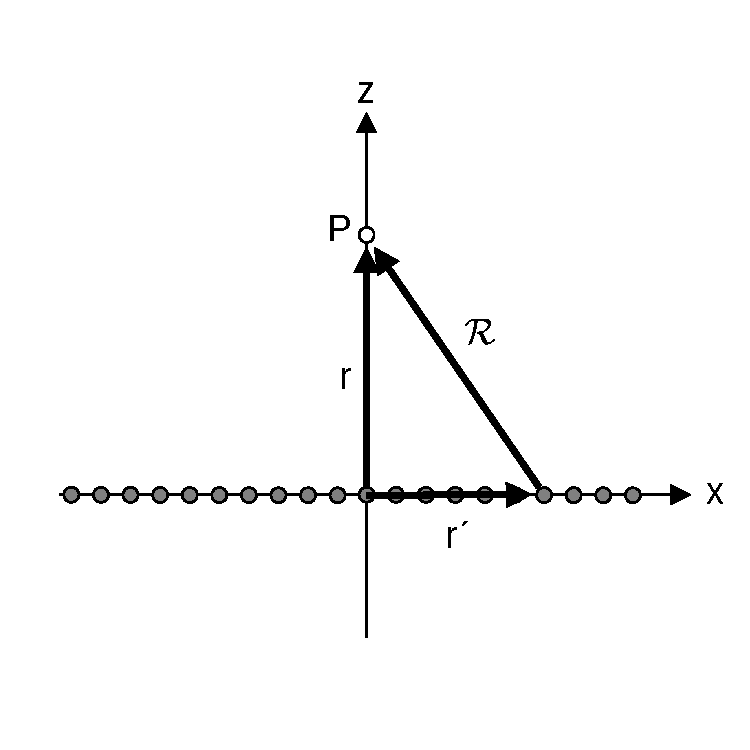
\includegraphics[width=8cm,trim=0cm 3cm 0cm 1cm,clip=true]{figures/line_of_charges.pdf}
\caption{\label{fig:line} A row of charges extends down the x-axis and the observer position is along the z-axis.}
\end{figure}
\end{frame}

\begin{frame}{The Line of Charges}
The voltage may be treated as sum of $2N + 1$ Coulomb potentials, with the origin treated separately.  Let
\begin{align}
V_0 &= \frac{1}{4\pi\epsilon_0} \frac{q}{z} \\
V_n &= \frac{1}{4\pi\epsilon_0} \frac{q}{\sqrt{z^2 + (n\Delta x)^2}}
\end{align}
\begin{equation}
V(z) = V_0 + 2 \sum_{n=1}^{N} V_n
\end{equation}
Let's examine the limit that $\alpha < 1$, where $\alpha = \Delta x / z$.
\end{frame}

\begin{frame}{The Line of Charges}
The potential at $z$ is
\begin{align}
V(z) &= \frac{1}{4\pi\epsilon_0} \frac{q}{z}\left( 1 + 2 \sum_{n=1}^{N} (1 + \alpha^2 n^2)^{-1/2} \right) \\
V(z) &\approx \frac{1}{4\pi\epsilon_0} \frac{q}{z}\left( 1 + 2 \sum_{n=1}^{N} \left(1 - \frac{1}{2} \alpha^2 n^2 \right) \right) \\
V(z) &\approx \frac{1}{4\pi\epsilon_0} \frac{q}{z}\left( 1 + 2N - \frac{2}{2} \alpha^2 \sum_{n=1}^N n^2 \right)  \\
V(z) &\approx \frac{q(2N+1)}{4\pi\epsilon_0 z}\left( 1 - \frac{\alpha^2}{(2N+1)} \sum_{n=1}^N n^2 \right)
\end{align}
\end{frame}

\begin{frame}{The Line of Charges}
The sum of the first $N$ squared integers is
\begin{equation}
\sum_{n=1}^{N} n^2 = \frac{N(N+1)(2N+1)}{6}
\end{equation}
The total charge $Q$ is $Q = q(2N+1)$.  Thus, $V(z)$ becomes
\begin{align}
V(z) &\approx \frac{Q}{4\pi\epsilon_0 z}\left( 1 - \frac{\alpha^2}{(2N+1)} \frac{N(N+1)(2N+1)}{6} \right) \\
V(z) &\approx \frac{Q}{4\pi\epsilon_0 z}\left( 1 - \frac{\alpha^2 N(N+1)}{6} \right) \label{eq:V_disc_1}
\end{align}
Suppose that $N \gg 1$, but such that $L = N\Delta x$ is constant.  In that case, $N(N+1) \approx N^2$.
\end{frame}

\begin{frame}{The Line of Charges}
Notice that
\begin{align}
N^2 \alpha^2 &= N^2 \left( \frac{\Delta x}{z} \right)^2 \\
N^2 \alpha^2 &= \left( \frac{N \Delta x}{z} \right)^2 \\
N^2 \alpha^2 &= \left( \frac{L}{2z} \right)^2 = \frac{L^2}{4 z^2} \label{eq:L}
\end{align}
Inserting Eq. \ref{eq:L} into Eq. \ref{eq:V_disc_1}:
\begin{equation}
V(z) \approx \frac{Q}{4\pi\epsilon_0 z}\left( 1 - \frac{L^2}{24 z^2} \right)
\end{equation}
\end{frame}

\begin{frame}{The Line of Charges}
Let $\beta_1 = L^2/24$.  The final result is
\begin{equation}
\boxed{
V(z) \approx \frac{Q}{4\pi\epsilon_0 }\left( \frac{1}{z} - \frac{\beta_1}{z^3} \right)
}
\end{equation}
Now to compare to the continuous case.  Let $dq = \lambda dx$, $\vec{r} = z \hat{z}$, and $\rcurs = \sqrt{z^2 + x^2}$.  Let the line of charge run from $-L/2$ to $L/2$.  Let $\theta_1$ be the angle between vertical and $\rcurs$ when $x = -L/2$, and $\theta_2$ for $x = L/2$.  By the usual methods:
\begin{equation}
V(z) = \frac{\lambda}{4\pi\epsilon_0}\int_{\theta_1}^{\theta_2} \sec\theta d\theta
\end{equation}
Symmetry allows:
\begin{equation}
V(z) = \frac{2\lambda}{4\pi\epsilon_0}\int_{0}^{\theta_2} \sec\theta d\theta
\end{equation}
\end{frame}

\begin{frame}{The Line of Charges}
Recall that $\sec\theta_2 = \rcurs/z$ and $\tan\theta_2 = L/2z$.  The result of integration is
\begin{equation}
V(z) = \frac{2\lambda}{4\pi\epsilon_0} \ln \left( \frac{\rcurs}{z} + \frac{L}{2z}\right)
\end{equation}
Using the definition $\rcurs = \sqrt{z^2 + x^2}$, the logarithm can be expanded in a series:
\begin{equation}
V(z) \approx \frac{2\lambda}{4\pi\epsilon_0} \left( \frac{L}{2z} - \frac{\epsilon L^3}{z^3}\right)
\end{equation}
The constant $\epsilon$ is $\epsilon = 0.0208 ... $  Letting $\beta_2 = 2\epsilon L^2$, and recognizing that $Q = \lambda L$, the final result is
\begin{equation}
\boxed{
V(z) \approx \frac{Q}{4\pi\epsilon_0} \left( \frac{1}{z} - \frac{\beta_2}{z^3}\right)
}
\end{equation}
\end{frame}

\begin{frame}{The Line of Charges}
\begin{figure}
\centering
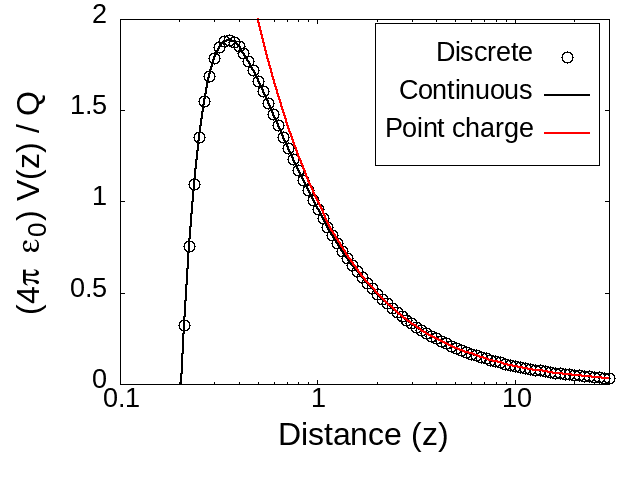
\includegraphics[width=8cm]{figures/line_of_charges.png}
\caption{\label{fig:line} The potential versus $z$ (in units of $Q/4\pi\epsilon_0$) for the discrete case (black circles), continuous linear density (black line), and a single point charge (red line).}
\end{figure}
\end{frame}

\section{Spatial Fourier transform}

\begin{frame}{Spatial Fourier transform}
What is the Fourier transform of $f(z)$?
\begin{equation}
f(z) = \frac{1}{z} - \frac{\beta}{z^3}
\end{equation}
Let the Fourier transform in question be $\mathcal{F}(f(z))_k$.  Relying on the linear property of Fourier transforms (indeed, all integrals), and consulting integral tables leads to the following:
\begin{align}
\mathcal{F}(f(z)) &= \mathcal{F}\left(\frac{1}{z}\right) - \beta \mathcal{F}\left(\frac{1}{z^3}\right) \\
\mathcal{F}\left(\frac{1}{z}\right) &= -i\pi \sign(k) \\
\mathcal{F}\left(\frac{1}{z^3}\right) &= -i\pi \frac{(-2i\pi k)^2}{2} \sign(k)
\end{align}
\end{frame}

\begin{frame}{Spatial Fourier transform}
Putting the pieces together, the magnitude of the spatial Fourier transform of $V(z)$ is
\begin{equation}
\boxed{
|\widetilde{V}(k)| = \frac{Q}{4\pi \epsilon_0} \pi \left( 1 + 2 \beta_{1,2} \pi^2 k^2 \right)
}
\end{equation}
\end{frame}

\begin{frame}{The Line of Charges}
\begin{figure}
\centering
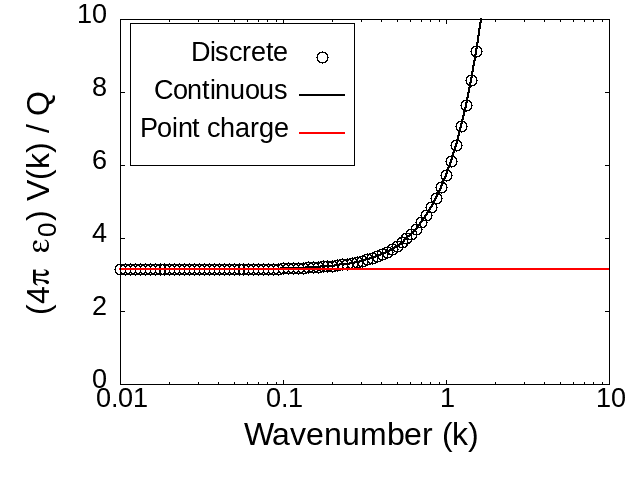
\includegraphics[width=8cm]{figures/line_of_charges2.png}
\caption{\label{fig:line2} The spatial Fourier transform of the potential versus $k$ (in units of $Q/4\pi\epsilon_0$) for the discrete case (black circles), continuous linear density (black line), and a single point charge (red line).}
\end{figure}
\end{frame}

\section{Summary}

\begin{frame}{Outline}
\begin{enumerate}
\item The continuous limit
\begin{itemize}
\item How accurate is the idea that $\Delta x \sum_i q_i \rightarrow \int dq$?
\item The spatial Fourier transform
\end{itemize}
\item The line of charges
\begin{itemize}
\item Discrete, continuous
\item Far-field approximation to third order in $(1/r)^n$
\item Spatial Fourier transforms
\end{itemize}
\end{enumerate}
\end{frame}

\end{document}
